%# -*- coding: utf-8-unix -*-
%%==================================================
\chapter{先进专家系统}\label{AIChapter10}
%%%%%%%%%%%%%%%%%%%%%%%%%%%%%%%%%%%%%%%%%%
%%%%%%%%%%%%%%%%%%%%%%%%%%%%%%%%%%%%
\begin{tcolorbox}[colback=white!50,colframe=orange!50,title=专家系统]
\begin{center}
专家系统是一个具有的专门知识与经验的程序系统, 它应用人工智能技术和计算机技术, 根据某领域一个或多个专家提供的知识和经验, 进行推理和判断, 模拟人类专家的决策过程, 以便解决那些需要人类专家处理的复杂问题。
专家系统是一个智能计算机程序系统, 其内部含有大量的某个领域专家水平的知识与经验, 能够利用人类专家的知识和解决问题的方法来处理该领域问题;是一种模拟人类专家解决领域问题的计算机程序系统。
\hfill
\end{center}
\end{tcolorbox}

\begin{figure}[H]
\centering

\includegraphics[width=0.76\textwidth]{AIExpert20191218.png}
\label{AIExpert20191218}
\end{figure}
%%%%%%%%%%%%%%%%%%%%%%%%%%%%%%%%%%%%%%%%%%

%%%%%%%%%%%%%%%%%%%%%%%%%%%%%%%%%%%%%%%%%%%%%%
\section{专家系统}
%%%%%%%%%%%%%%%%%%%%%%%%%%%%%%%%%%%%%%%%%%%%%%
\subsection{专家系统概述}
专家系统和先进专家系统

专家系统的概念

    专家系统是一种具有大量专门知识和经验的智能程序系统, 它能运用领域专家多年积累的经验和专门知识, 模拟领域专家的思维过程, 解决该领域中需要专家才能解决的复杂问题.

先进专家系统的概念

    先进专家系统是指在传统专家系统的基础上, 引入一些新思想、新技术所产生的新型专家系统.

先进专家系统的特性

    (1) 并行分布式处理功能

    (2) 多专家协同工作

    (3) 更强的自学习能力

    (4) 更新的推理机制

    (5) 自纠错和自完善能力

    (6) 先进的智能接口

    (7) 更多的先进技术被引入和融合

%%%%%%%%%%%%%%%%%%%%%%%%%%%%%%%%%%%%%
\subsection{专家系统的基本结构}
尽管不同类型的专家系统的结构会存在一定差异, 但其基本结构还是大致相同的. 通常, 一个专家系统的基本结构由知识库、数据库、推理机、解释模块、知识获取模块和人机接口6大部分所组成. 如图\ref{Expertbase20191203}所示:
%%%%%%%%%%%%%%%%%%%%%%%%%%%%%%%%%%%%%%%%%%
\begin{figure}[H]
\centering
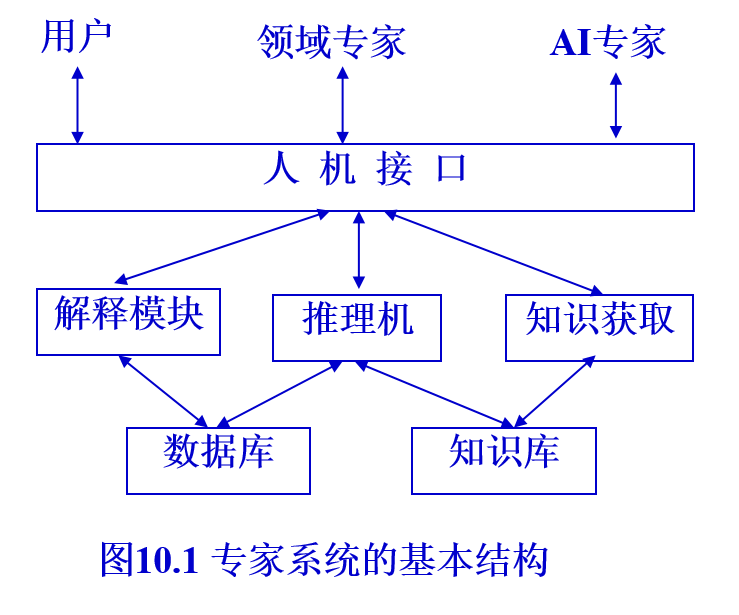
\includegraphics[width=0.76\textwidth]{Expertbase20191203.png}
\caption{模糊专家系统}
\label{Expertbase20191203}
\end{figure}
%%%%%%%%%%%%%%%%%%%%%%%%%%%%%%%%%%
%%%%%%%%%%%%%%%%%%%%%%%%%%%%%%%%%%%%%%%%%%%%%%
\subsection{基于规则和基于框架的专家系统}
基于规则的专家系统是指采用产生式知识表示方法的专家系统. 它以产生式系统为基础, 是专家系统开发中常用的一种方式, 其最基本的工作模型如图\ref{Expertbase20191303}所示.
%%%%%%%%%%%%%%%%%%%%%%%%%%%%%%%%%%%%%%%%%%
\begin{figure}[H]
\centering

\includegraphics[width=0.76\textwidth]{Expertbase20191303.png}
\caption{模糊专家系统}
\label{Expertbase20191303}
\end{figure}
%%%%%%%%%%%%%%%%%%%%%%%%%%%%%%%%%%
在该模型中, 规则库是基于规则专家系统的知识库;事实库也称综合数据库, 是用来存放推理前的已知事实和推理过程中所得到的中间结论的;推理机是基于规则专家系统的推理机构.

基于框架的专家系统是指采用框架知识表示方法的专家系统. 它以框架系统为基础, 具有较好的结构化特性. 这种专家系统的基本结构也与图\ref{Expertbase20191203}所示的专家系统类似, 其主要区别在于知识库中知识表示和组织方式, 综合数据库中事实的表示方式, 推理机的推理方法和系统推理过程的控制策略等.
%%%%%%%%%%%%%%%%%%%%%%%%%%%%%%%%%%%%%%%%%%%%%%
\subsection{模糊专家系统和神经网络专家系统}
%%%%%%%%%%%%%%%%%%%%%%%%%%%%%%%%%%%%%
\subparagraph{模糊专家系统}
模糊专家系统是指采用模糊技术来处理不确定性的一类专家系统. 模糊专家系统的基本结构与传统专家系统类似, 一般由模糊知识库、模糊数据库、模糊推理机、知识获取模块、解释模块和人机接口6部分所组成. 如图\ref{Expertbase20191403}:
%%%%%%%%%%%%%%%%%%%%%%%%%%%%%%%%%%%%%%%%%%
\begin{figure}[H]
\centering
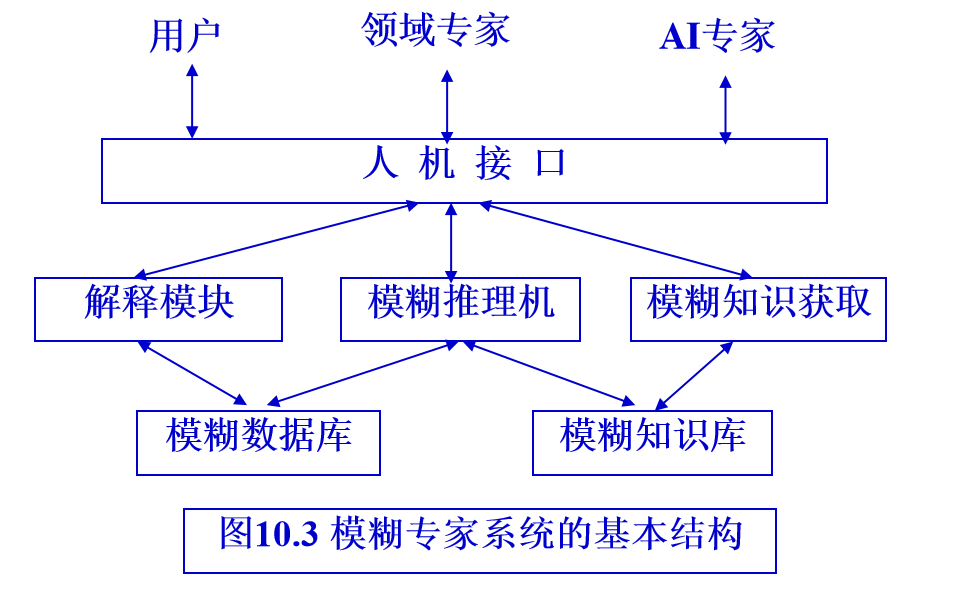
\includegraphics[width=0.76\textwidth]{Expertbase20191403.png}
\caption{模糊专家系统}
\label{Expertbase20191403}
\end{figure}
%%%%%%%%%%%%%%%%%%%%%%%%%%%%%%%%%%
%%%%%%%%%%%%%%%%%%%%%%%%%%%%%%%%%%%%%
\subparagraph{神经网络专家系统}
神经网络专家系统是神经网络与传统专家系统集成所得到的一种专家系统. 它将传统专家系统的显式的知识表示方法变为基于神经网络及其连接权值的隐式知识表示, 把基于逻辑的串行推理技术变为基于神经网络的并行联想和自适应推理.
%%%%%%%%%%%%%%%%%%%%%%%%%%%%%%%%%%%%%%%%%%%%%%
\subsection{基于Web的专家系统}
    基于Web的专家系统是Web数据交换技术与传统专家系统集成所得到的一种先进专家系统. 它利用Web浏览器实现人机交互, 基于Web专家系统中的各类用户都可通过浏览器访问专家系统. 从结构上, 它由浏览器、应用服务器和数据库服务器三个层次所组成, 包括Web接口、推理机、知识库、数据库和解释器.
%%%%%%%%%%%%%%%%%%%%%%%%%%%%%%%%%%%%%%%%%%%%%%
\subsection{分布式专家系统和协同式专家系统}
这是两种不同的先进专家系统, 它们各自的侧重点不一样. 分布式专家系统强调并行和分布, 而协同式专家系统则强调协作与协同.
%%%%%%%%%%%%%%%%%%%%%%%%%%%%%%%%%%%%
\subparagraph{分布式专家系统}
分布式专家系统(Distributed Expert System, DES)是具有并行分布处理特征的专家系统, 它可以把一个专家系统的功能分解后, 分布到多个处理机上去并行执行, 从而在总体上提高系统的处理效率. 其运行环境可以是紧密耦合的多处理器系统, 也可以是松耦合的计算机网络环境.
%%%%%%%%%%%%%%%%%%%%%%%%%%%%%%%%%%%%
\subparagraph{协同式专家系统}
协同式专家系统(Cooperative Expert System, CES)亦称群专家系统, 是一种能综合若干个相近领域或同一领域内不同方面专家系统相互协作、共同解决单个专家系统无法解决的更广领域或更复杂问题的专家系统.

从结构上它们有一定的相似之处, 它们都涉及到多个分专家系统. 但在功能上却有较大差异, 分布式专家系统强调的是功能分布和知识分布, 它要求系统必须在多个节点上并行运行;而协调式专家系统强调的则是各专家系统之间的协同, 各分专家系统可以在不同节点上运行, 也可以在同一个节点上运行.
%%%%%%%%%%%%%%%%%%%%%%%%%%%%%%%%%%%%%%%%%%%%%%
\section{专家系统的开发}
%%%%%%%%%%%%%%%%%%%%%%%%%%%%%%%%%%%%
\paragraph{开发步骤}
采用原型技术的专家系统开发过程如下图所示, 它可分为设计初始知识库、原型系统开发与试验、知识库的改进与归纳三个主要步骤.
%%%%%%%%%%%%%%%%%%%%%%%%%%%%%%%%%%%%
\paragraph{知识获取}

%%%%%%%%%%%%%%%%%%%%%%%%%%%%%%%%%%%%
\paragraph{输入知识}

%%%%%%%%%%%%%%%%%%%%%%%%%%%%%%%%%%%%
\paragraph{开发工具与环境}
常用的专家系统开发工具和环境可按其性质分为程序设计语言、骨架型工 具、语言型工具、开发环境及一些新型专家系统开发工具等.
\begin{itemize}
\item 程序设计语言
    程序设计语言包括人工智能语言和通用程序设计语言. 它们是专家系统开发的最基础的语言工具. 人工智能语言的主要代表有以LISP为代表的函数型语言和以PROLOG为代表的逻辑型语言等;通用程序设计语言的主要代表有C、C++和JAVA等.
\item 骨架型工具
    骨架型工具也称为专家系统外壳, 它是由一些已经成熟的具体专家系统演变来的. 其演变方法是, 抽去这些专家系统中的具体知识, 保留它们的体系结构和功能, 再把领域专用的界面改为通用界面, 这样, 就可得到相应的专家系统外壳.
\item 语言型工具
    语言型工具是一种通用型专家系统开发工具, 它是不依赖于任何已有专家系统, 不针对任何具体领域, 完全重新设计的一类专家系统开发工具. 与骨架系统相比, 语言型工具具有更大的灵活性和通用性, 并且对数据及知识的存取和查询提供了更多的控制手段. 常用的语言型工具有CLIPS和OSP等.
\item 开发环境
\end{itemize}
    专家系统开发环境是一种为高效率开发专家系统而设计和实现的大型智能计算机软件系统. 专家系统开发环境一般由调试辅助工具、输入输出设施、解释设施和知识编辑器4个典型部件所组成.

%%%%%%%%%%%%%%%%%%%%%%%%%%%%%%%%%%%%%%%%%%%%%%
\section{作 业}
%%%%%%%%%%%%%%%%%%%%%%%%%%%%%%%%%%%%%%%%%%%%%%%%
\begin{think}
先进专家系统有哪些主要特征?它有哪些主要类型?
\end{think}
%%%%%%%%%%%%%%%%%%%%%%%%%%%%%%%%%%%%%%%%%%%%%%%%
\begin{think}
什么是分布式专家系统?什么是协同式专家系统?它们的主要区别是什么?
\end{think}
